
\section{Cấu hình hệ thống}
%====================================================================================

\subsection{Cấu hình hệ thống PLC và module}
Công cụ lập trình dùng cho PLC Mitsubishi Q Series là phần mềm GX Works2.
Khi khởi tạo project cần chọn dòng PLC (Q mode); loại CPU (Q13UDV); loại project (Simple Project) và ngôn ngữ lập trình sử dụng trong project (Ladder). Cấu hình như Hình \ref{c3:newprj}.

Sau khi đã tạo thành công project mới, cần cấu hình hệ thống PLC tương ứng với phần cứng sử dụng. 
\begin{figure} [h]
    \centering
    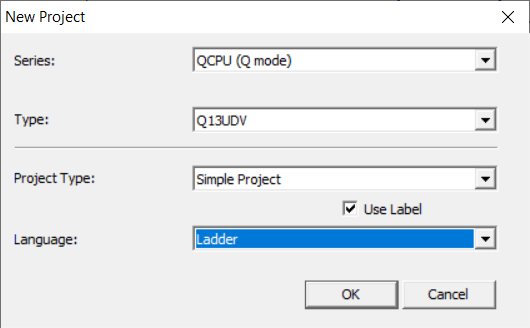
\includegraphics[width=0.75\linewidth]{figures/Chapter3/newprj.png}
    \caption{Cấu hình New Project}
    \label{c3:newprj}
\end{figure}
%\newpage
\begin{enumerate}
    \item Cấu hình base unit và các module giống với thiết lập phần cứng như Hình \ref{c3:hardware}. 
    Thiết lập thông tin của base unit và vị trí module trong GX Works2 như Hình \ref{c3:io} tại \textit{Parameter} $\rightarrow$ \textit{PLC Parameter} $\rightarrow$ \textit{I/O Assignment}.
    \begin{figure}[H]
    \centering
    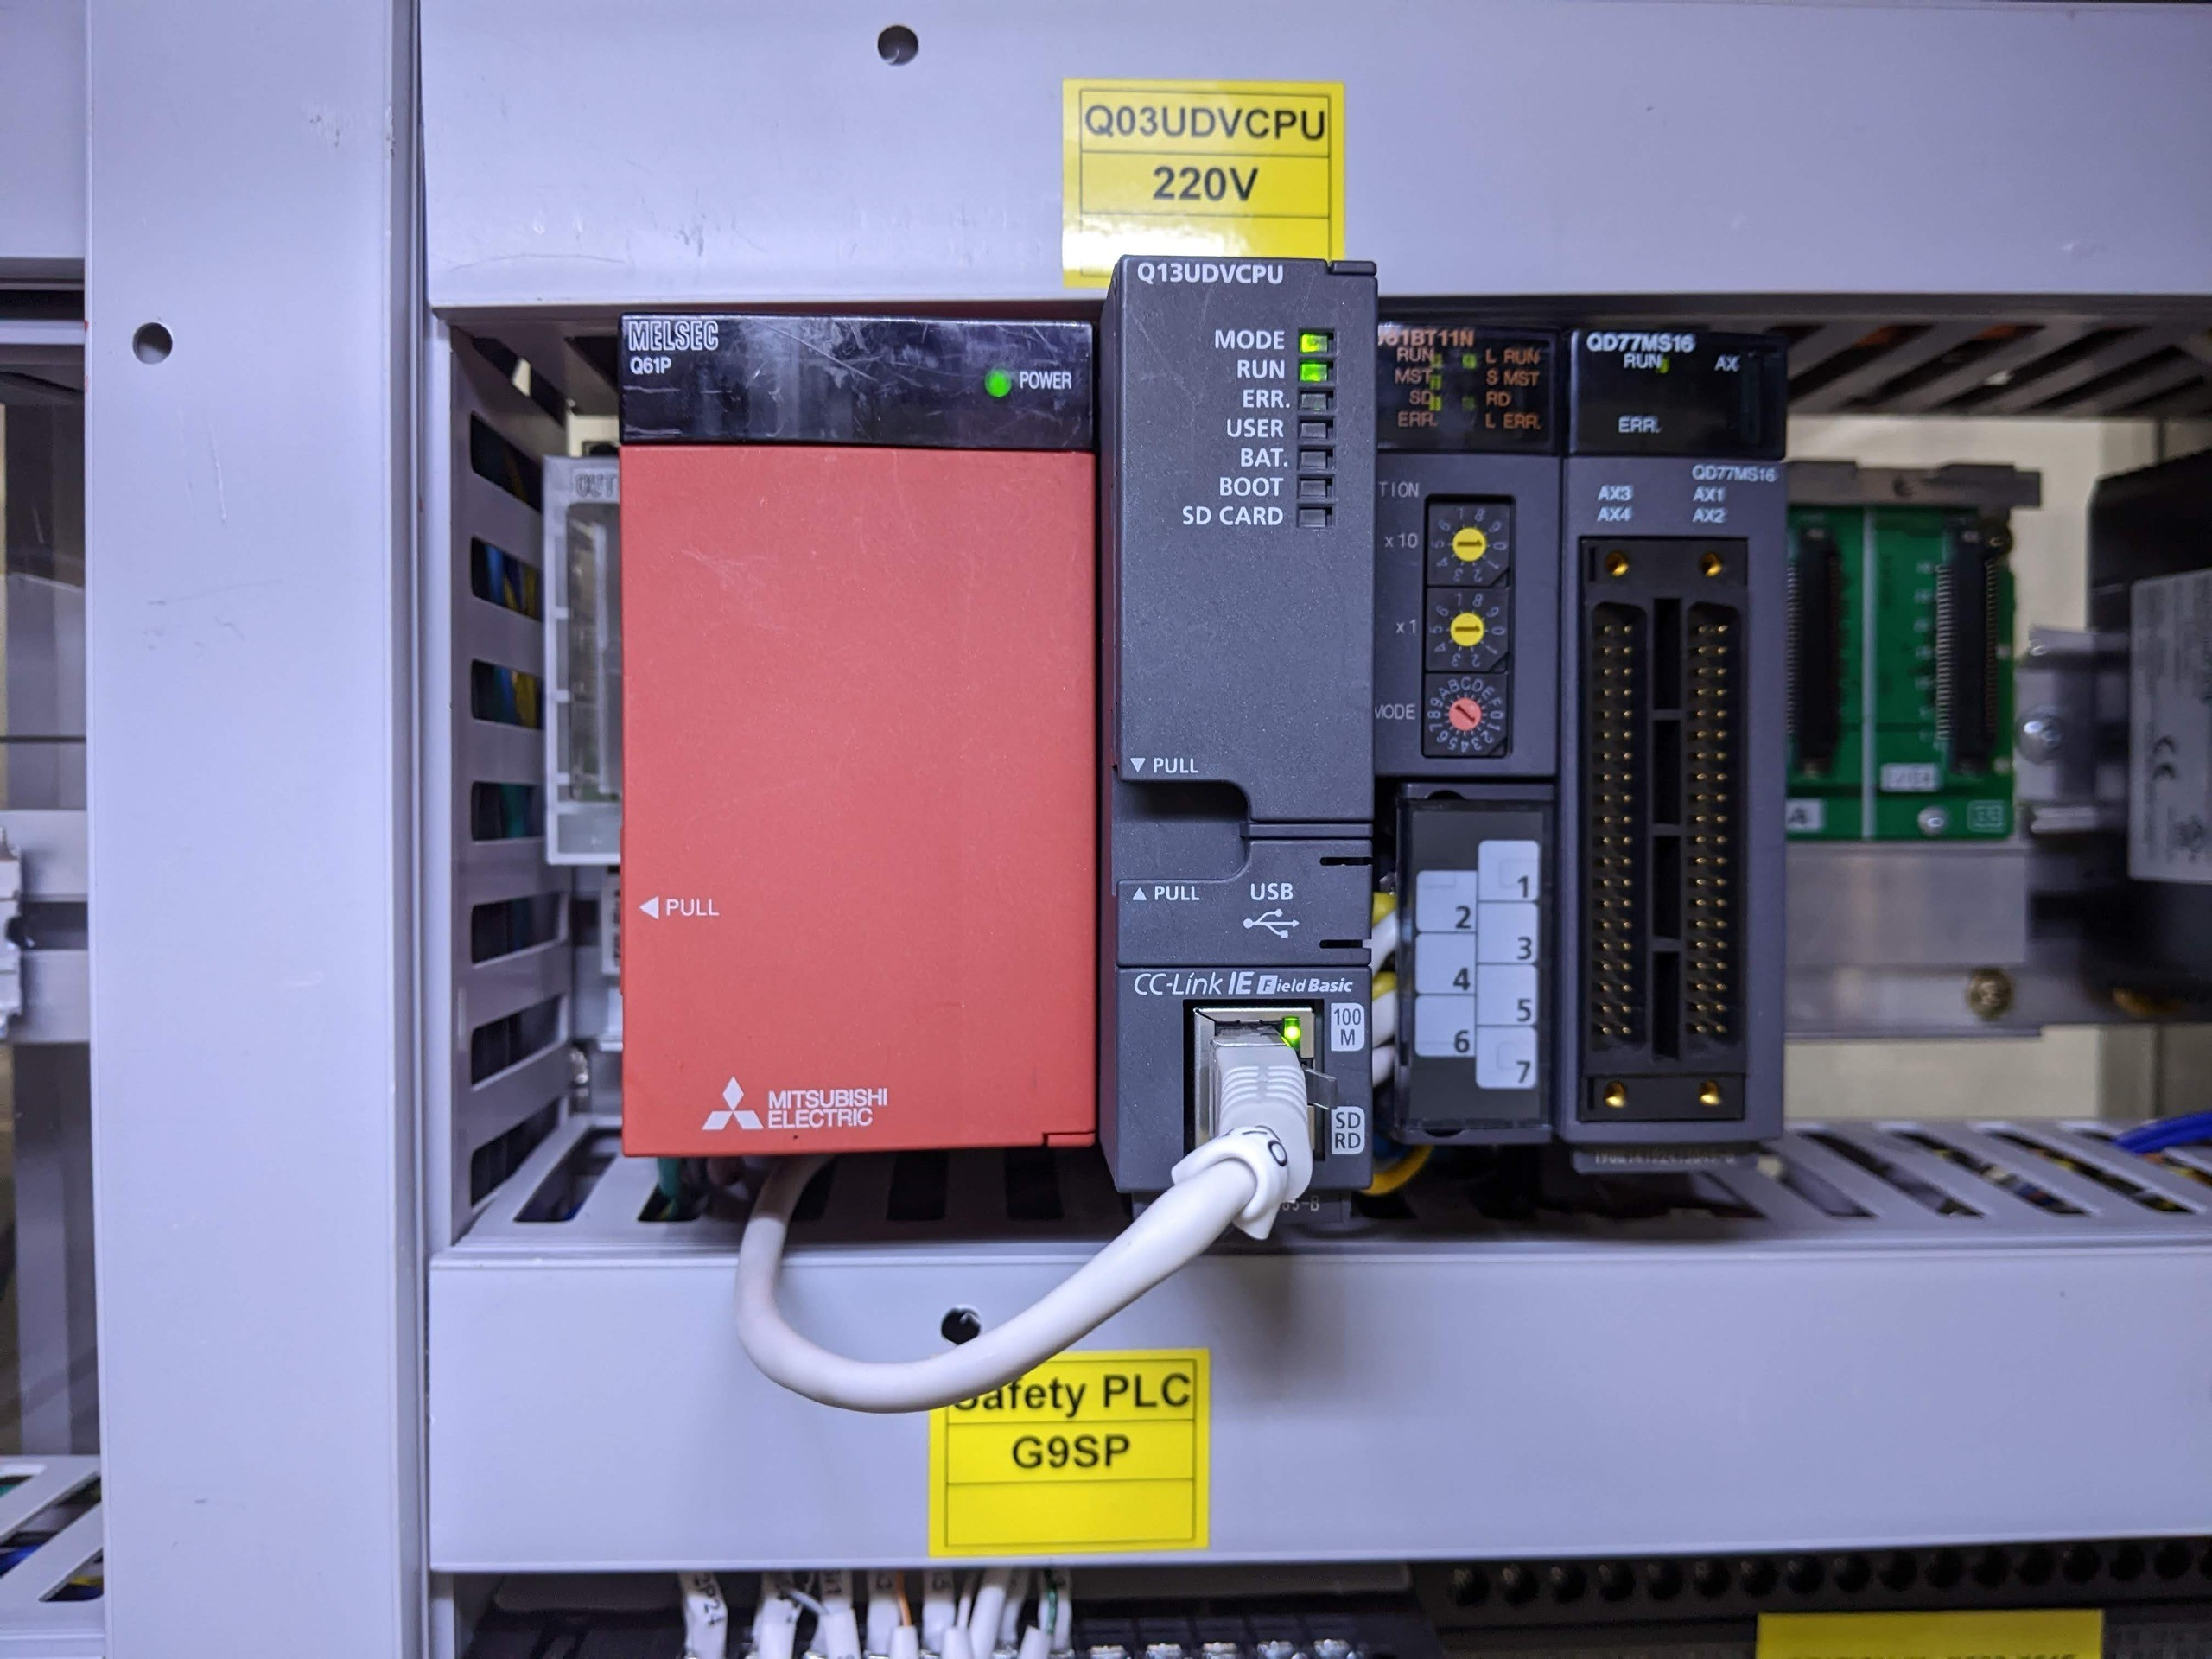
\includegraphics[width=0.75\linewidth]{figures/Chapter3/phancung.png}
    \caption{Thiết lập phần cứng}
    \label{c3:hardware}
    \end{figure}

    
    \begin{figure}[H]
        \centering
        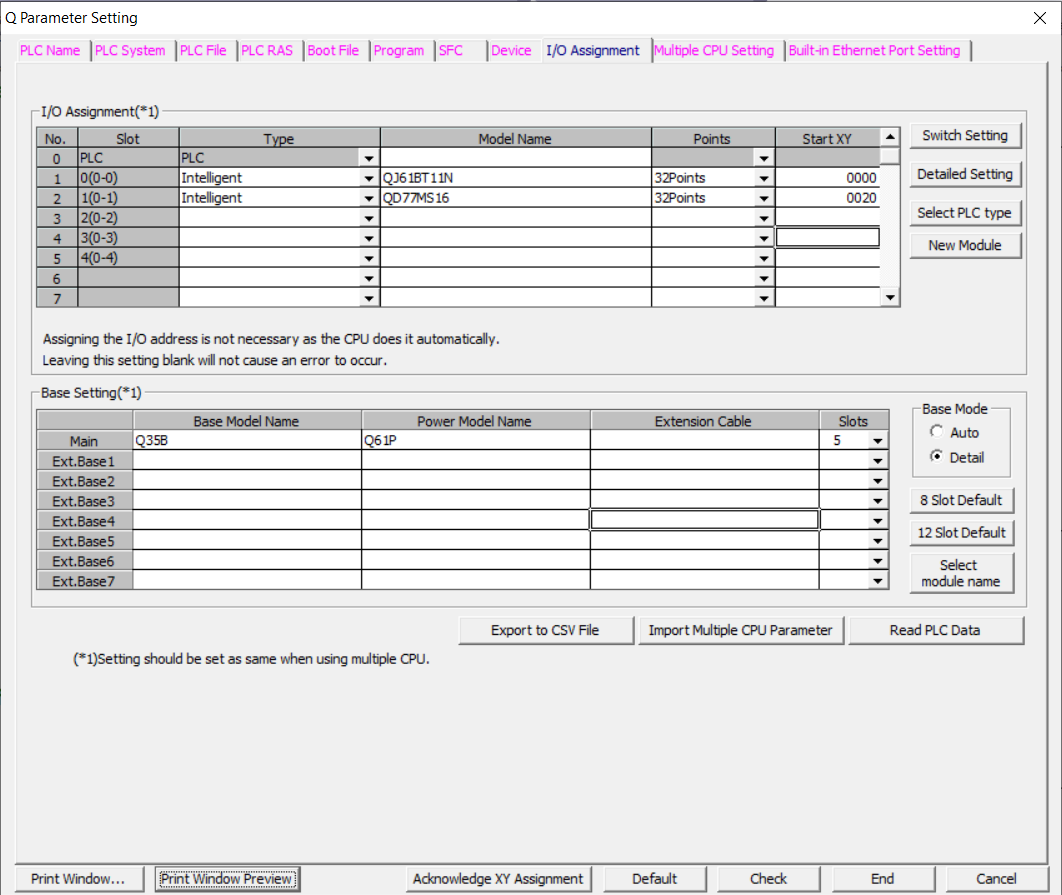
\includegraphics[width=0.75\linewidth]{figures/Chapter3/io.png}
        \caption{IO Assignment}
        \label{c3:io}
    \end{figure}

    \item Cấu hình giao tiếp/kết nối giữa PLC với GX Works2 (PC Side) như Hình \ref{c3:ethernet}. Bao gồm thiết lập IP cho PLC, giao thức MC Protocol.
    \begin{figure}[H]
        \centering
        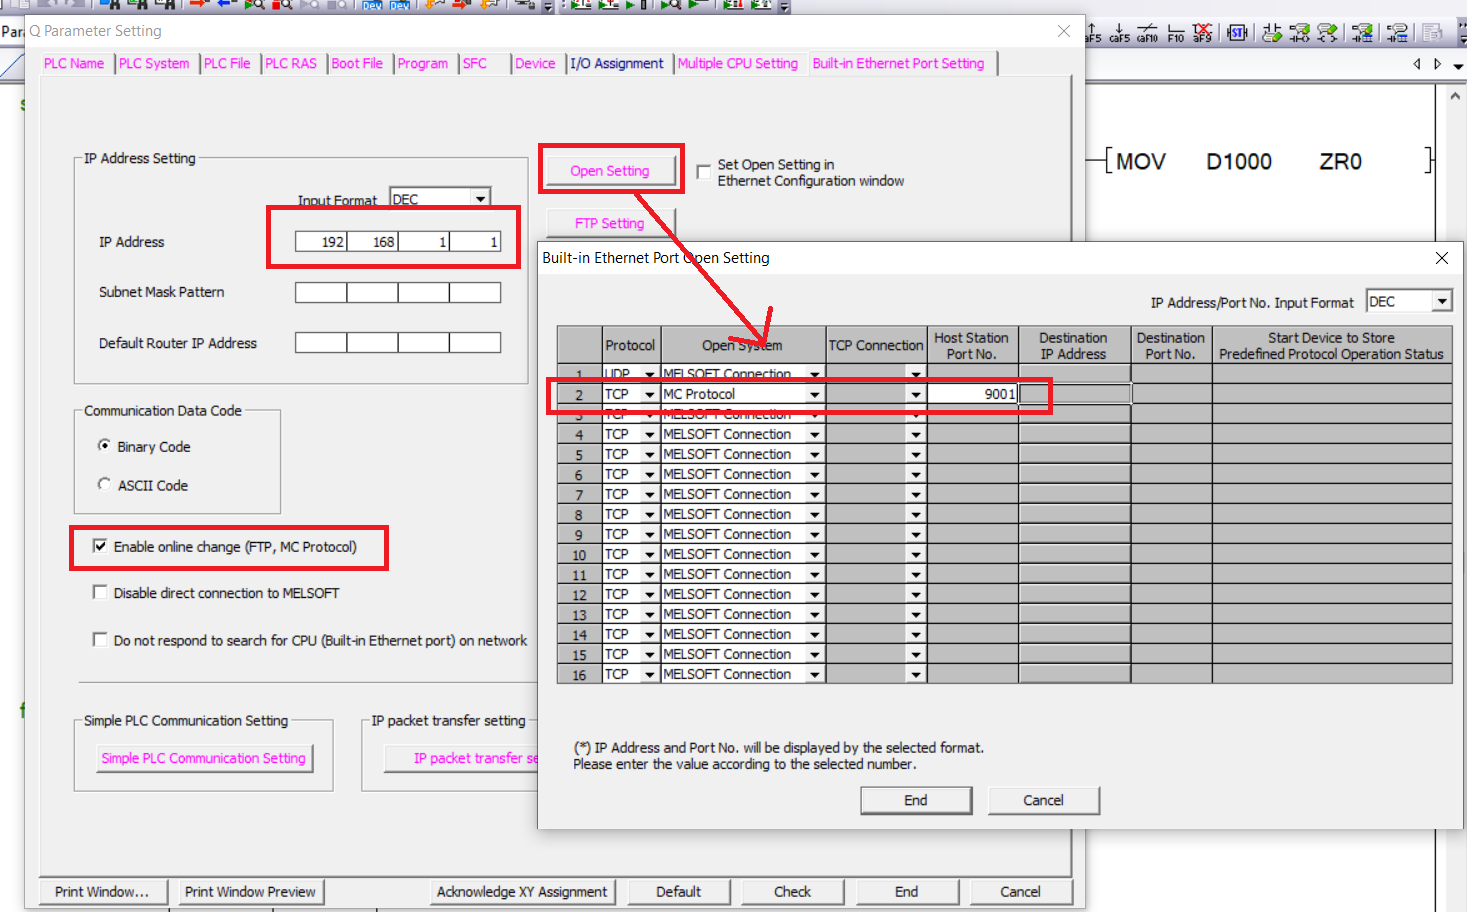
\includegraphics[width=0.75\linewidth]{figures/Chapter3/ethernet.png}
        \caption{Thiết lập kết nối Ethernet}
        \label{c3:ethernet}
    \end{figure}  
\end{enumerate}
Sau khi kết thúc thiết lập, bấm End để lưu thiết lập.

 \subsection{Cấu hình CC-Link giao tiếp giữa PLC và các CC-Link Station}

Để có thể kết nối các trạm với PLC qua CC-Link cần thiết lập cả phần cứng và phần mềm.
Cần cấu hình hai thông số quan trọng là phiên bản CC-Link (Ver 2 hoặc Ver 1), tốc độ truyền (khoảng cách càng gần thì tốc độ càng cao), số thứ tự Station cho từng trạm (cả Remote IO và Remote Device).

\begin{enumerate}
    \item \textbf{Trạm I/O}: Cấu hình các trạm IO là Remote IO Station. 
    Hình minh họa phần cứng của Remote IO giống như Hình \ref{c3:remoteio}. Có hai thành phần quan trọng là công tắc định địa chỉ Station (3) và công tắc định tốc độ giao tiếp (2). Cần phải điều khiển sao cho tốc độ đúng với tốc độ hệ thống và địa chỉ phù hợp, không bị trùng với các trạm khác.
        
    \begin{figure}[H]
        \centering
        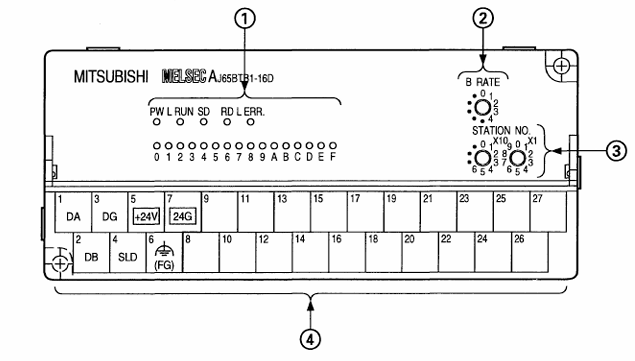
\includegraphics[width=0.75\linewidth]{figures/Chapter3/remote-io.png}
        \caption{Phần cứng Remote IO}
        \label{c3:remoteio}
    \end{figure}  

    \item \textbf{Robot Hyundai}: Cấu hình robot là Remote Device Station.
    Để có thể giao tiếp với mạng CC-Link, cần gắn thêm board giao tiếp CC-Link BD570 vào bộ điều khiển, minh họa như Hình\ref{c3:cc1}.
    \begin{figure}[H]
        \centering
        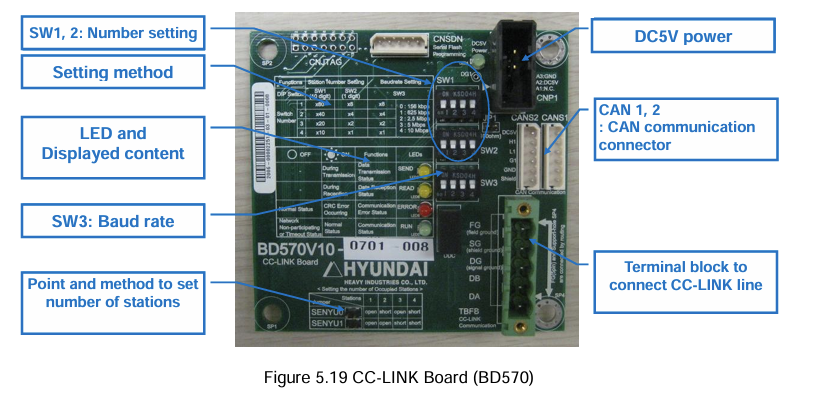
\includegraphics[width=1\linewidth]{figures/Chapter3/h-cc.png}
        \caption{Board CC-Link}
        \label{c3:cc1}
    \end{figure}
    Gắn board CC-Link vào bộ điều khiển, sau đó thiết lập vị trí trạm và tốc độ truyền bằng các switch có trên board.
    Sau khi bật nguồn bộ điều khiển, thông tin về giao tiếp CC-Link được hiển thị bằng Teach pendant (Hình \ref{c3:cc2}).
    \begin{figure}[H]
        \centering
        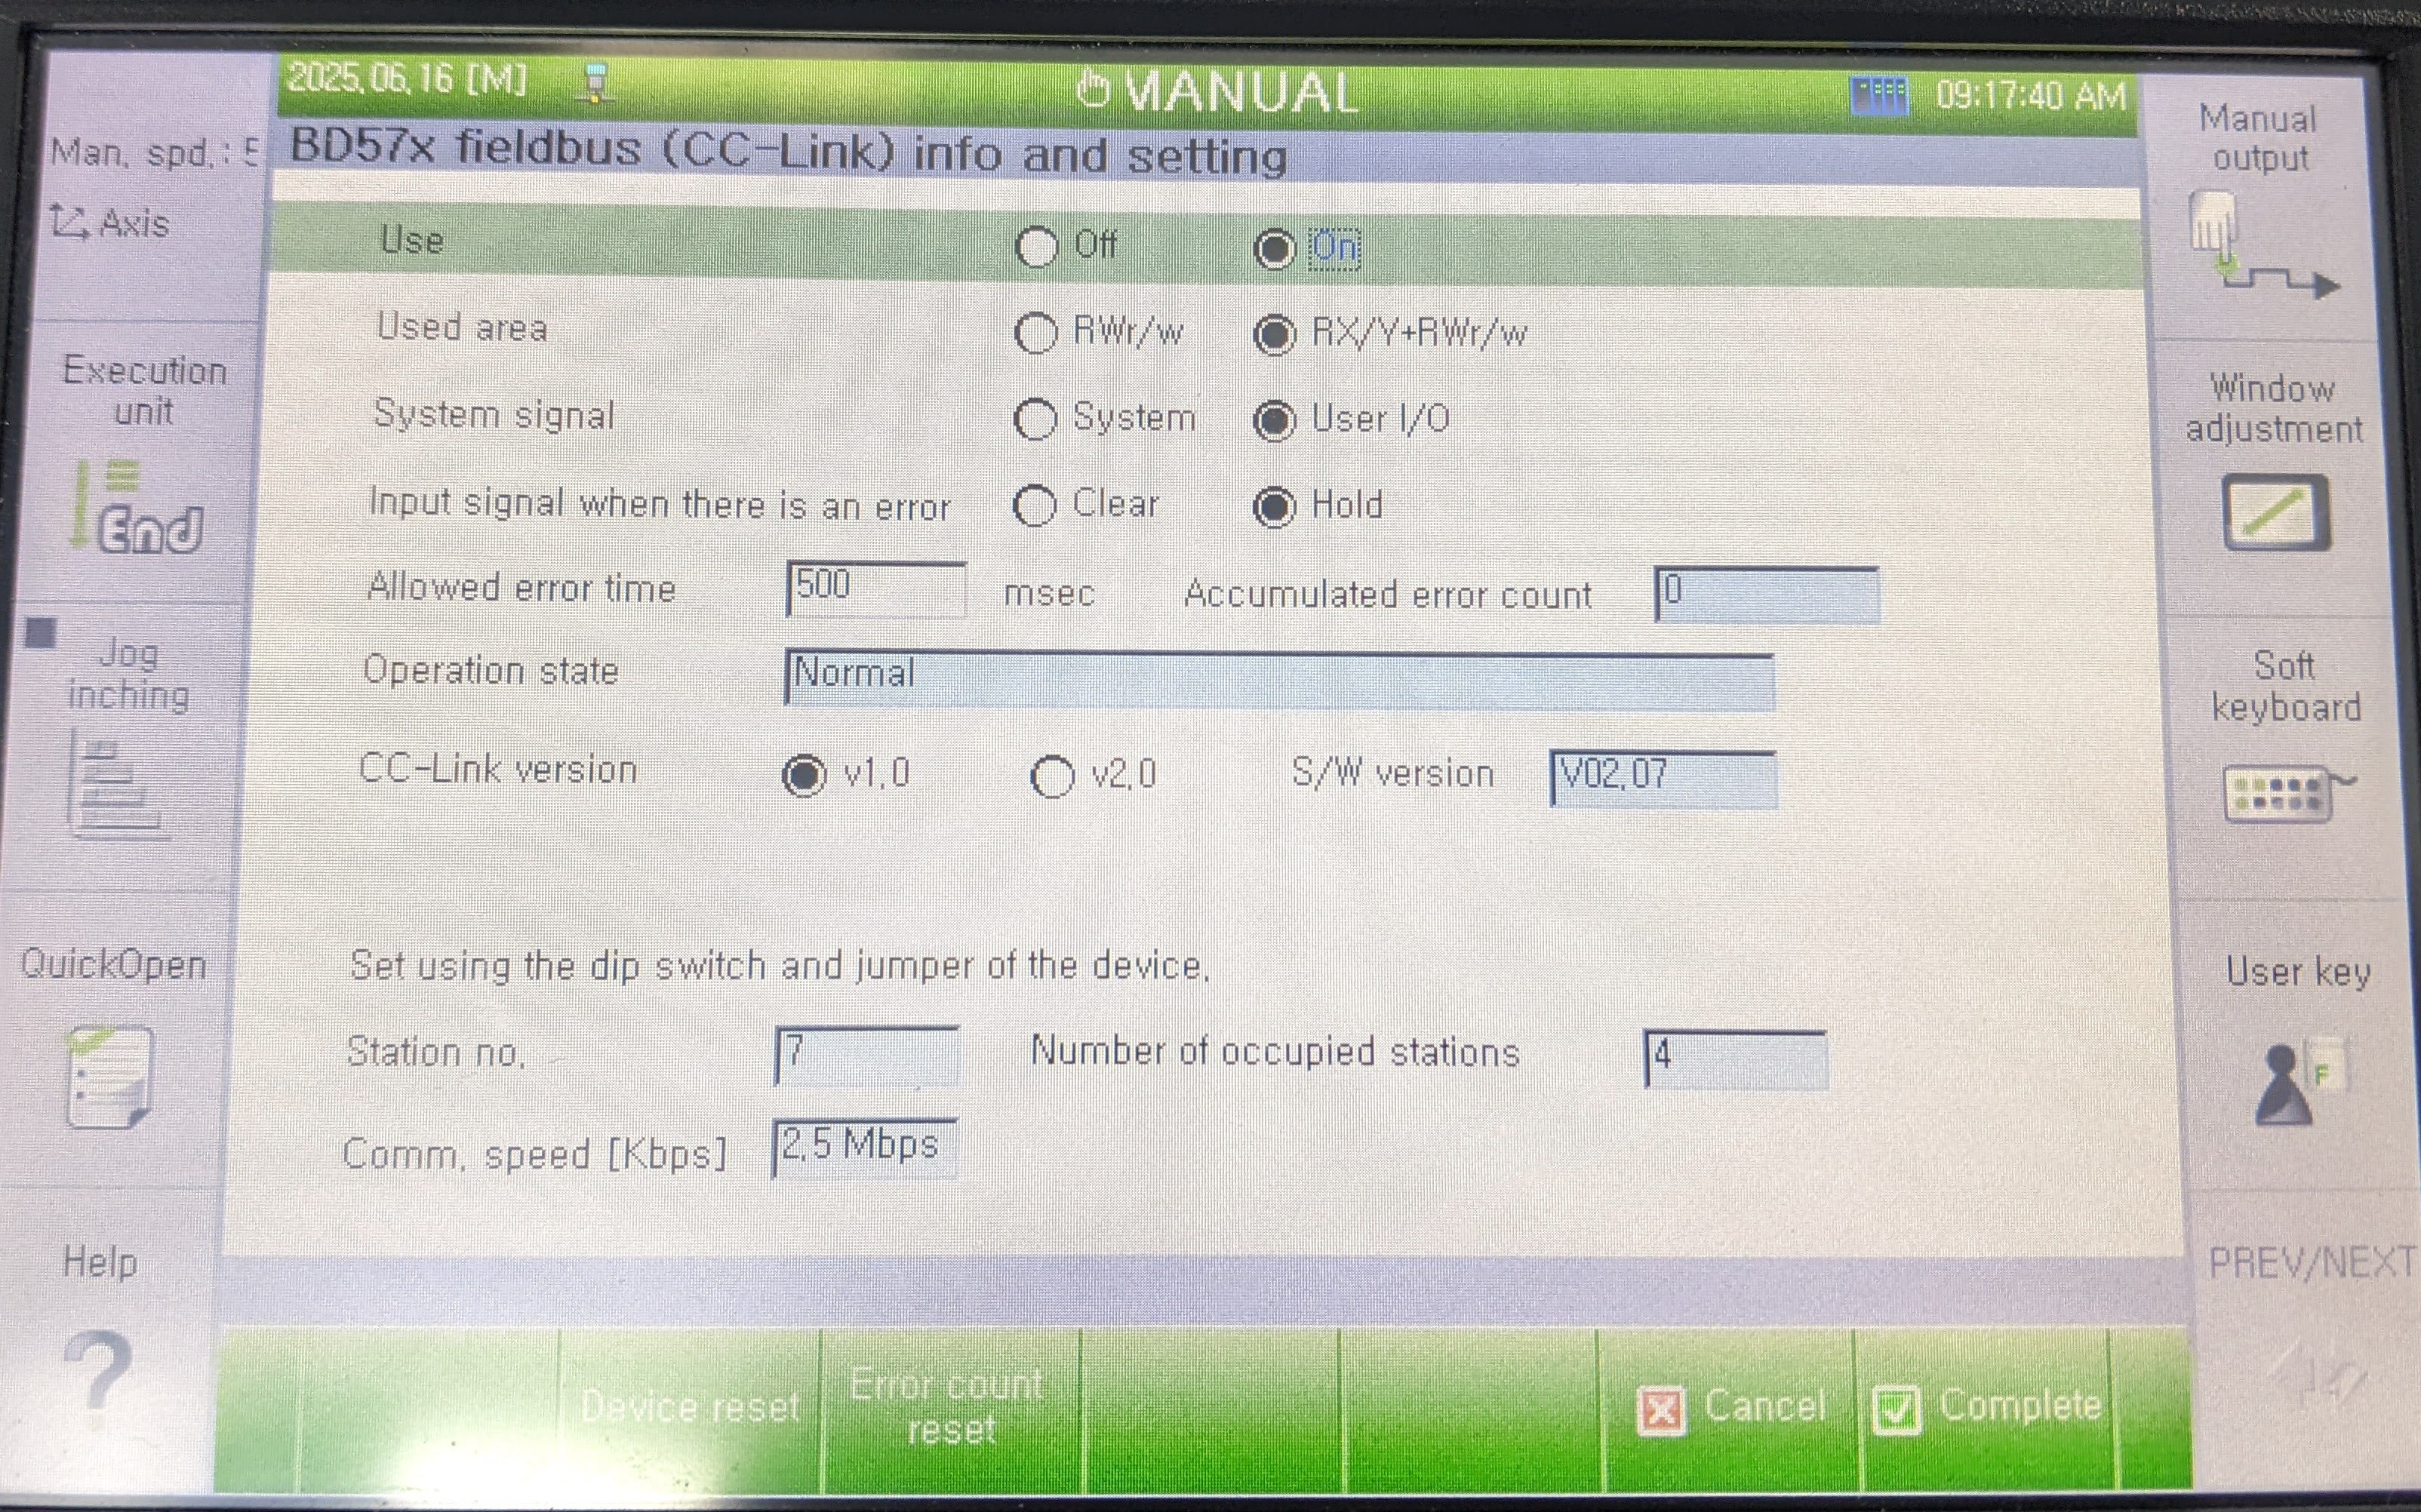
\includegraphics[width=1\linewidth]{figures/Chapter3/h-cc2.jpg}
        \caption{Thiết lập CC-Link Robot Hyundai}
        \label{c3:cc2}
    \end{figure}
    Thông số cấu hình CC-Link của Robot Hyundai:
    \newline
    \begin{tabular}{lc}
        \toprule
        \midrule
        Station no. & 7 \\
        Number of occupied stations & 4 \\
        Communication speed & 2.5 Mbps \\
        CC-Link version & v1.0 \\
        \bottomrule
    \end{tabular}

 Sau khi cấu hình xong, dữ liệu từ CC-Link được hiển thị tại 
\texttt{F1:Service} $\rightarrow$ 
\texttt{1:Monitoring} $\rightarrow$ 
\texttt{3:Field bus signal} $\rightarrow$ 
\texttt{9/10:FB5 Field bus input/output}.



    \newpage
    \item \textbf{Robot Yaskawa}: Cấu hình robot là Remote Device Station. 
    Để có thể kết nối Robot với PLC qua CC-Link giúp truyền nhận tín hiệu In/Out và Register, cần phải lắp đặt phần cứng là CCS-PCIE Board (Hình \ref{c3:yas2})vào bộ điều khiển của Robot YRC1000micro.
    \begin{figure}[H]
        \centering
        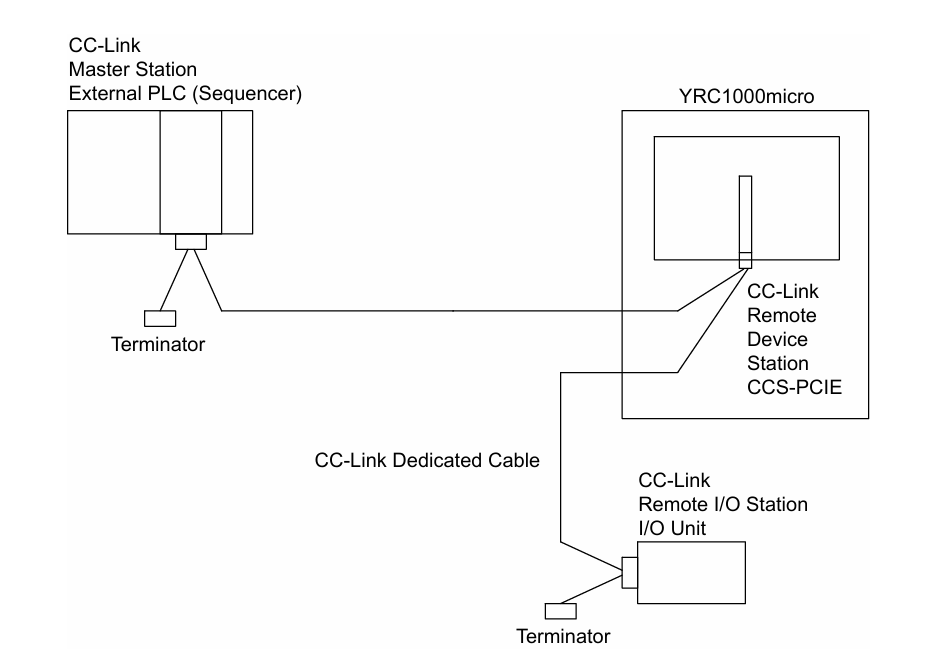
\includegraphics[width=0.8\linewidth]{figures/Chapter3/yas1.png}
        \caption{Kết nối CC-Link giữa Robot Yaskawa và PLC}
        \label{c3:yas1}
    \end{figure}
    

    \begin{figure}[H]
        \centering
        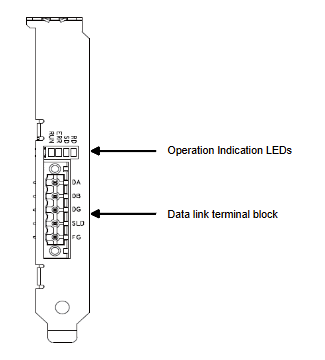
\includegraphics[width=0.5\linewidth]{figures/Chapter3/y-cc1.png}
        \caption{Board CCS-PCIE}
        \label{c3:yas2}
    \end{figure}

    Thiết lập giao tiếp CC-Link cần vào Maintenance Mode: nhấn \texttt{[MAIN MENU]} trong khi bật nguồn YRC1000micro.  
    Sau đó thiết lập thông tin cho Board CCS-PCIE như dưới:
    \begin{figure}[H]
        \centering
        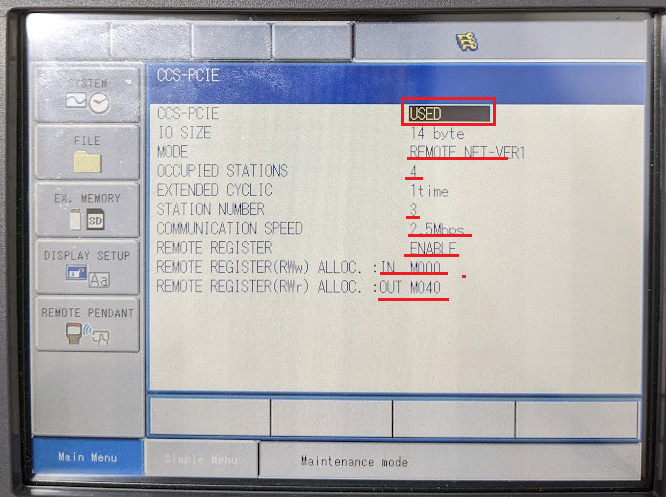
\includegraphics[width=1\linewidth]{figures/Chapter3/cclink1.png}
        \caption{Thiết lập CC-Link Robot Yaskawa}
        \label{c3:yas3}
    \end{figure}

    Thông số cấu hình CC-Link của Robot Yaskawa:
    \newline
        \begin{tabular}{lc}
            \toprule
            \midrule
            Station no. & 3 \\
            Number of occupied stations & 4 \\
            Communication speed & 2.5 Mbps \\
            CC-Link version & v1.0 \\
            IO Size & 14 bytes \\
            \bottomrule
        \end{tabular}

    Ấn \texttt{[ENTER]} đến màn hình \textit{EXTERNAL IO SETUP}:
    \begin{figure}[H]
        \centering
        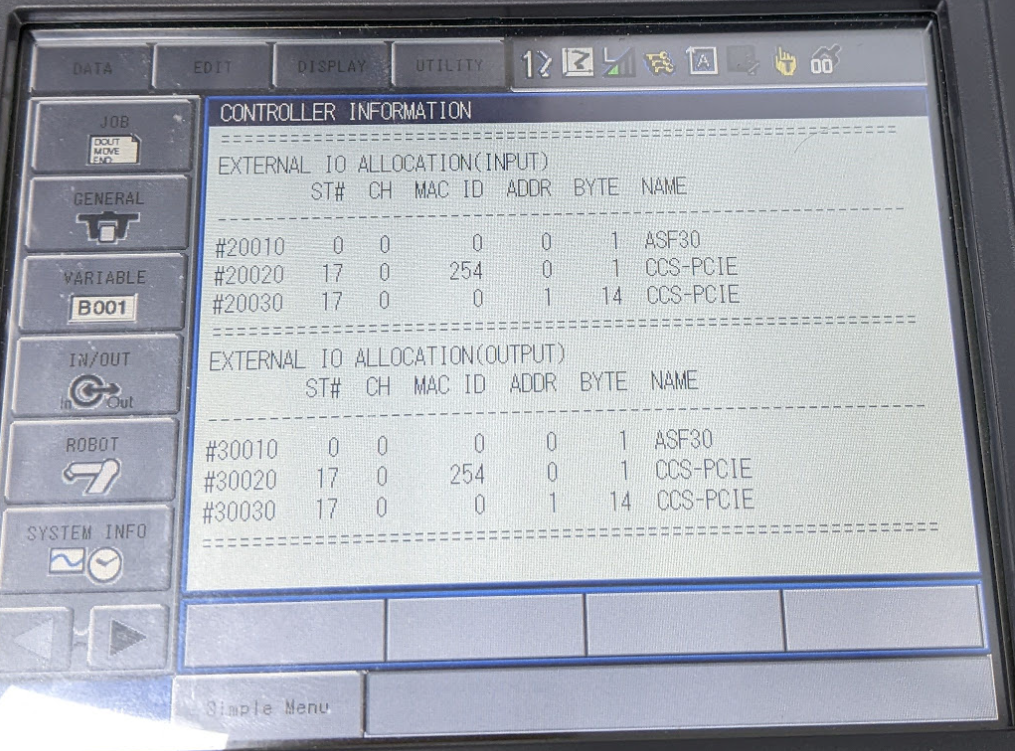
\includegraphics[width=1\linewidth]{figures/Chapter3/y-cc3.png}
        \caption{Controller Information}
        \label{c3:yas4}
    \end{figure}

    Hệ thống có ba loại dữ liệu vào/ra như sau:

    \begin{enumerate}
        \item \textbf{Dữ liệu từ board ASF30}:
        \begin{itemize}
            \item 8-bit input: \#20010–\#20017
            \item 8-bit output: \#30010–\#30017
        \end{itemize}

        \item \textbf{Dữ liệu trạng thái từ board CCS-PCIE}:
        \begin{itemize}
            \item 8-bit input: \#20020–\#20027
            \item 8-bit output: \#30020–\#30027
        \end{itemize}

        \item \textbf{Dữ liệu qua mạng CC-Link}:
        \begin{itemize}
            \item 14-byte input: \#20030–\#20167
            \item 14-byte output: \#30030–\#30167
        \end{itemize}
    \end{enumerate}

    Sau khi thiết lập dữ liệu từ CC-Link sang Robot, có thể kiểm tra tại  
    \texttt{[MAIN MENU]} $\rightarrow$ \texttt{IN/OUT} $\rightarrow$ \texttt{EXTERNAL INPUT/OUTPUT}.

    Để có thể sử dụng dữ liệu IO từ \texttt{EXTERNAL INPUT/OUTPUT} khi lập trình Robot cần chuyển vào \texttt{GENERAL PURPOSE INPUT/OUTPUT} \cite{YaskawaYRC1000microConcurrentIO} bằng cách sử dụng Ladder Program \cite{YaskawaYRC1000microOperatorManual}.

    \begin{figure}[H]
        \centering
        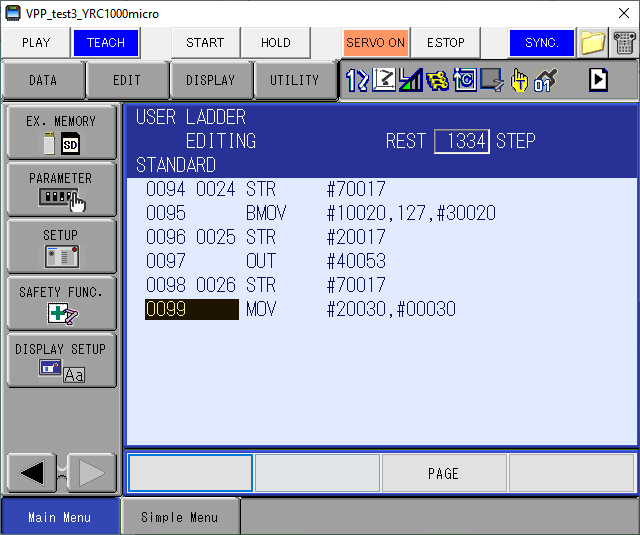
\includegraphics[width=1\linewidth]{figures/Chapter3/yas4.png}
        \caption{Ladder Program}
        \label{c3:yas5}
    \end{figure}

    \begin{figure}[H]
        \centering
        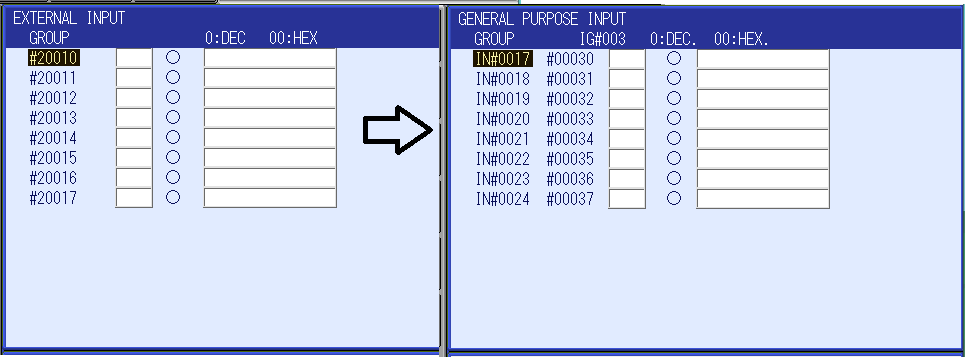
\includegraphics[width=1\linewidth]{figures/Chapter3/yas5.png}
        \caption{Dữ liệu chuyển vào GP INPUT/OUTPUT}
        \label{c3:yas6}
    \end{figure}

    Ví dụ: tại dòng 98–99, \texttt{\#20030 – \#20037} của \texttt{External Input} được chuyển vào \texttt{\#00030–\#00037} của \texttt{General Purpose Input}.

    \item \textbf{Cấu hình PLC là Master}

    Trong mục thiết lập tham số CC-Link của GX-Works2, cấu hình như sau:

    Thiết lập thông tin trạm Master (Hình \ref{c3:plc1} và Hình \ref{c3:plc2})

    \begin{figure}[H]
        \centering
        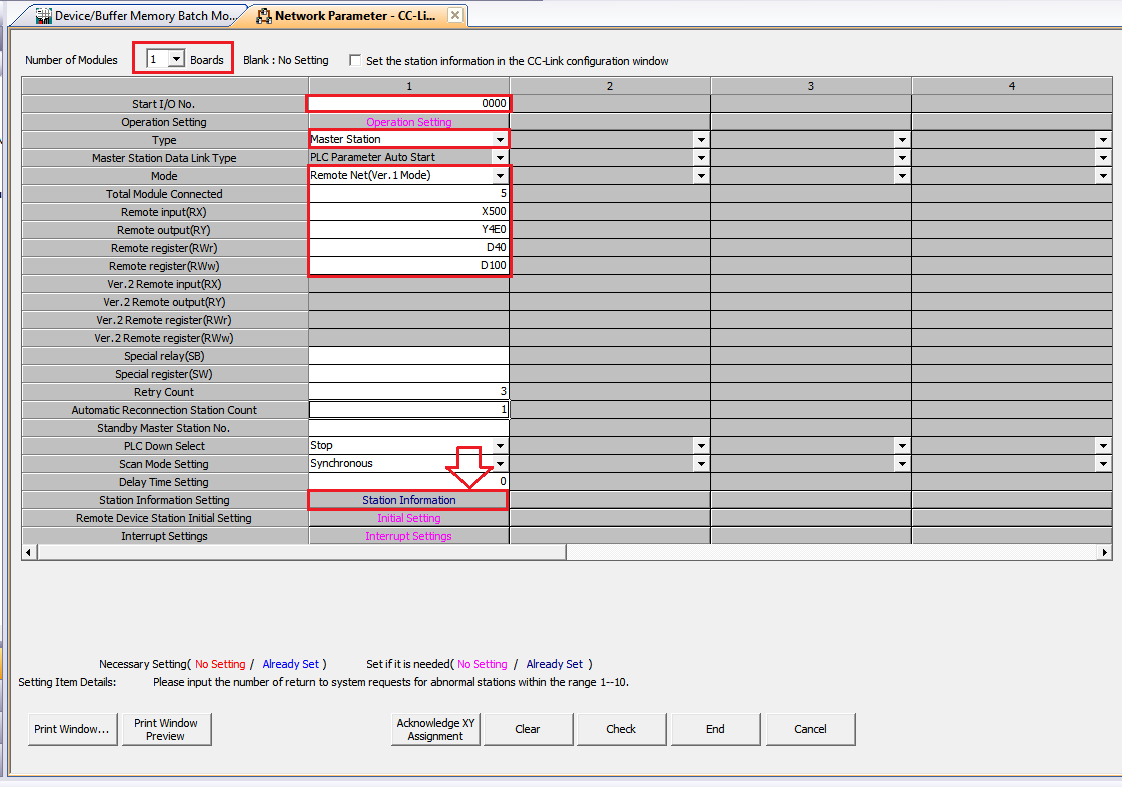
\includegraphics[width=0.9\linewidth]{figures/Chapter3/plc-cc1.png}
        \caption{Master Station}
        \label{c3:plc1}
    \end{figure}

    \begin{figure}[H]
        \centering
        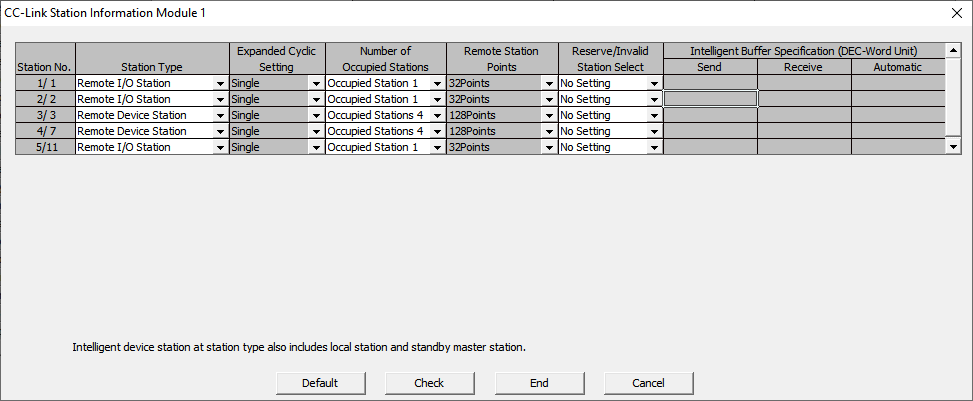
\includegraphics[width=1\linewidth]{figures/Chapter3/plc-cc2.png}
        \caption{Master Station Setup}
        \label{c3:plc2}
    \end{figure}

    \begin{figure}[H]
        \centering
        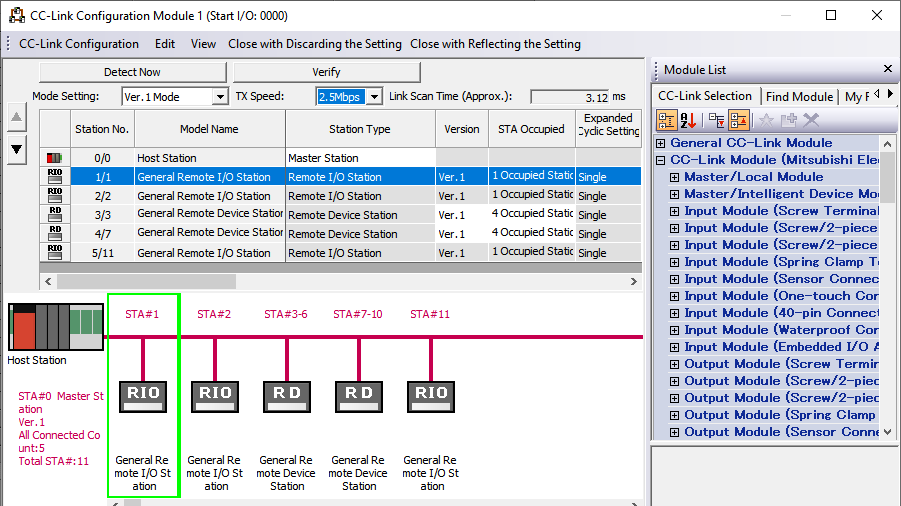
\includegraphics[width=1\linewidth]{figures/Chapter3/plc-cc3.png}
        \caption{CC-Link Speed}
        \label{c3:plc3}
    \end{figure}

    Sau khi thiết lập xong Master, thu được kết quả:

    \begin{itemize}
        \item Station \#1: AJ65SBTB1-32D
        \item Station \#2: AJ65SBTB1-32T1
        \item Station \#3: Robot Yaskawa (4 trạm)
        \item Station \#4: Robot Hyundai (4 trạm)
        \item Station \#5: AJ65SBT1-16DT1
    \end{itemize}

    Mỗi trạm chiếm:
    \begin{itemize}
        \item 32 bit tại Rx, Ry
        \item 4 word tại RWr, RWw
    \end{itemize}

    \begin{table}[h]
    \centering
    \begin{tabularx}{\textwidth}{|c|X|X|X|X|}
    \hline
    \textbf{Station} & \textbf{Rx} & \textbf{Ry} & \textbf{RWr} & \textbf{RWw} \\ \hline
    \#1 & X500--X51F & Y4E0--Y4FF & D40--D43 & D100--D103 \\ \hline
    \#2 & X520--X53F & Y500--Y51F & D44--D47 & D104--D107 \\ \hline
    \#3 & X540--X5BF & Y520--Y59F & D48--D63 & D108--D123 \\ \hline
    \#4 & X5C0--X63F & Y5A0--Y61F & D64--D79 & D124--D139 \\ \hline
    \#5 & X640--X65F & Y620--Y63F & D80--D83 & D140--D143 \\ \hline
    \end{tabularx}
    \caption{Bảng phân phối bit/word CC-Link}
    \label{tab:cclink}
    \end{table}


\end{enumerate}
%=------------------------------------------------------------------------------
\subsection{Cấu hình KepserverEX làm server OPC UA}
Kết nối KepserverEX với PLC qua card mạng của máy tính. Giao thức được chọn và sử dụng trong phần mềm GX-Works2 và phần mềm KepserverEX phải giống nhau để đảm bảo giao tiếp giữa OPC UA Server với PLC.

\begin{figure}[H]
        \centering
        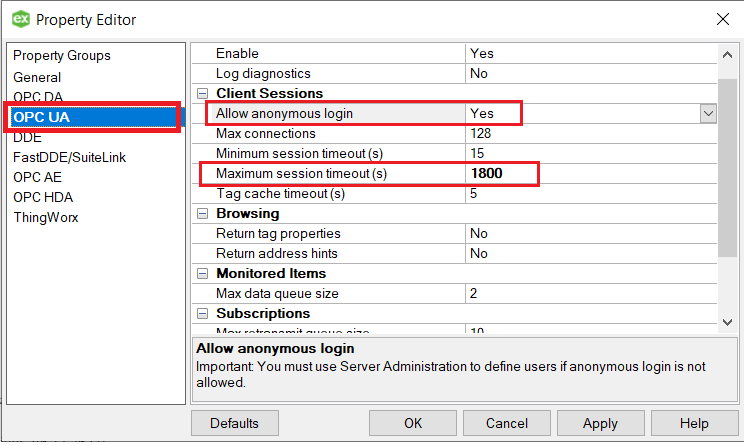
\includegraphics[width=1\linewidth]{figures/Chapter3/kepwareprj.png}
        \caption{Cấu hình Project Kepware}
        \label{c3:kepwareprj}
 \end{figure}

Cấu hình Project của Kepware như Hình \ref{c3:kepwareprj}, lưu ý bật cho phép truy cập ẩn danh.


\begin{figure}[H]
        \centering
        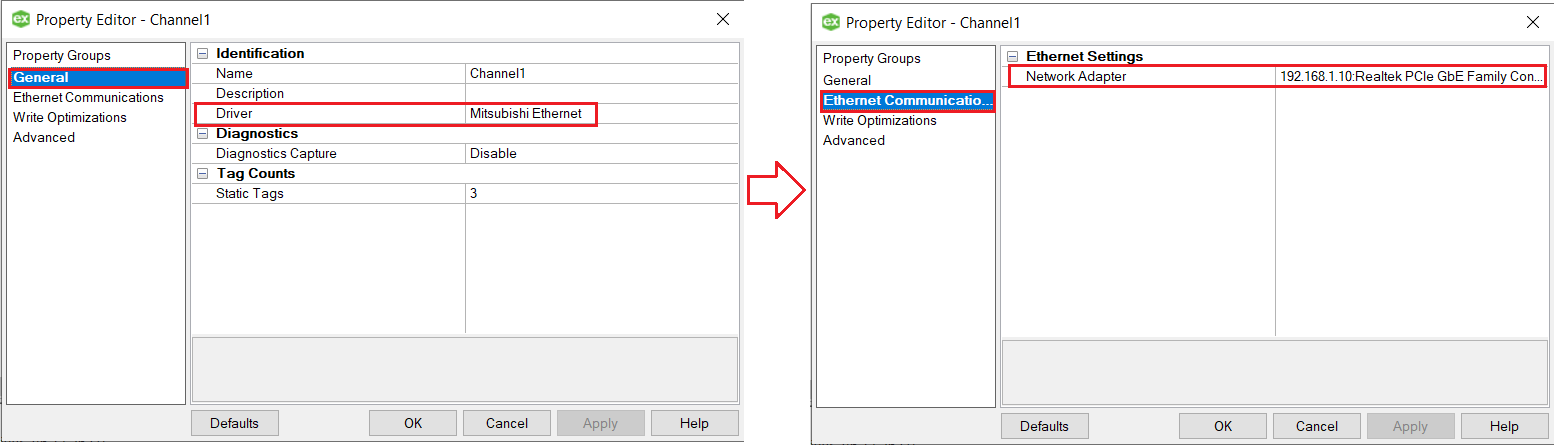
\includegraphics[width=1\linewidth]{figures/Chapter3/kepwarechannel.png}
        \caption{Cấu hình Channel}
        \label{c3:kepwarechannel}
 \end{figure}

Cấu hình Channel của Kepware project, lưu ý đúng với cổng mạng đang dùng của máy tính.

\begin{figure}[H]
        \centering
        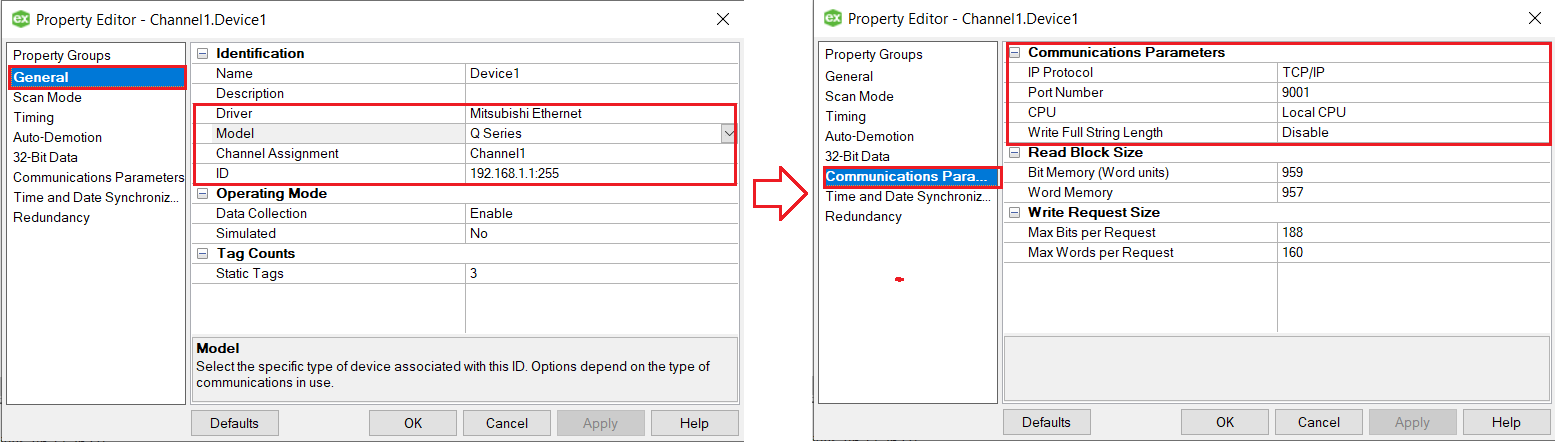
\includegraphics[width=1\linewidth]{figures/Chapter3/kepwaredevice.png}
        \caption{Cấu hình Device}
        \label{c3:kepwaredevice}
 \end{figure}

Cấu hình Device của Channel, lưu ý đúng với IP của PLC.

Tiếp theo cần tạo các Tag muốn sử dụng, tương ứng với địa chỉ các bit/word trong PLC


\subsection{Cấu hình GigE Camera Basler ac2500}
Kết nối Camera với máy tính qua cổng mạng IP, cần cấu hình IP của camera với IP của máy tính trong cùng lớp mạng (Hình \ref{c3:cameraip}).

\begin{figure}[H]
        \centering
        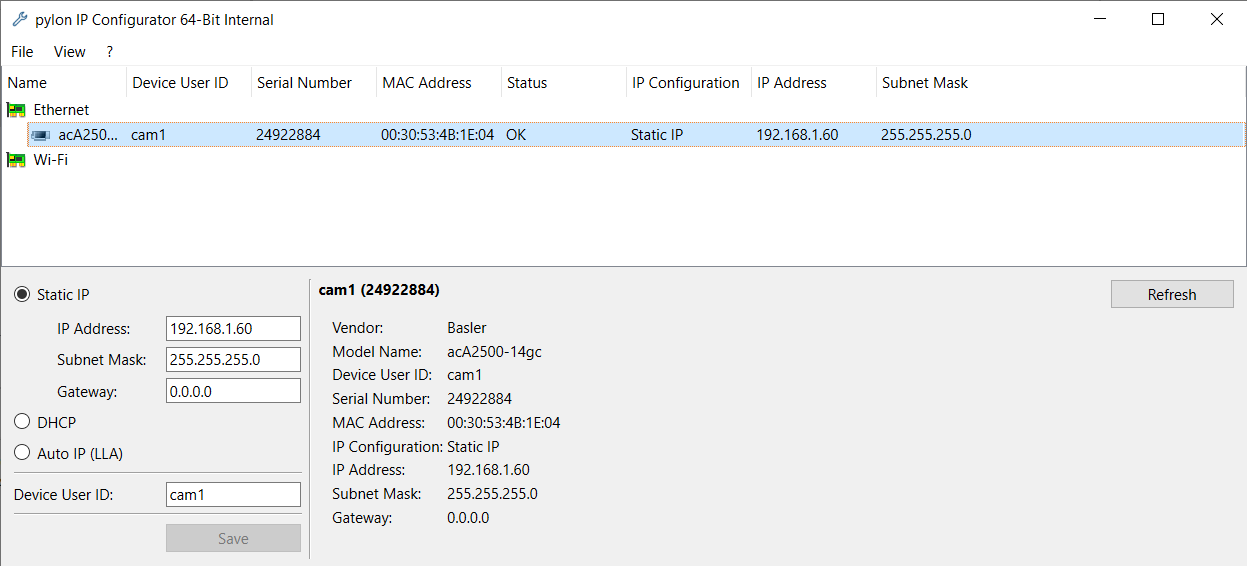
\includegraphics[width=1\linewidth]{figures/Chapter3/baslerip.png}
        \caption{Cấu hình IP camera}
        \label{c3:cameraip}
 \end{figure}

Tiếp theo là cấu hình thông số ảnh chụp như Gain, Gamma, Exposure time. Có thể sử dụng chức năng Automatic Image Adjustment (Hình \ref{c3:image}).

\begin{figure}[H]
        \centering
        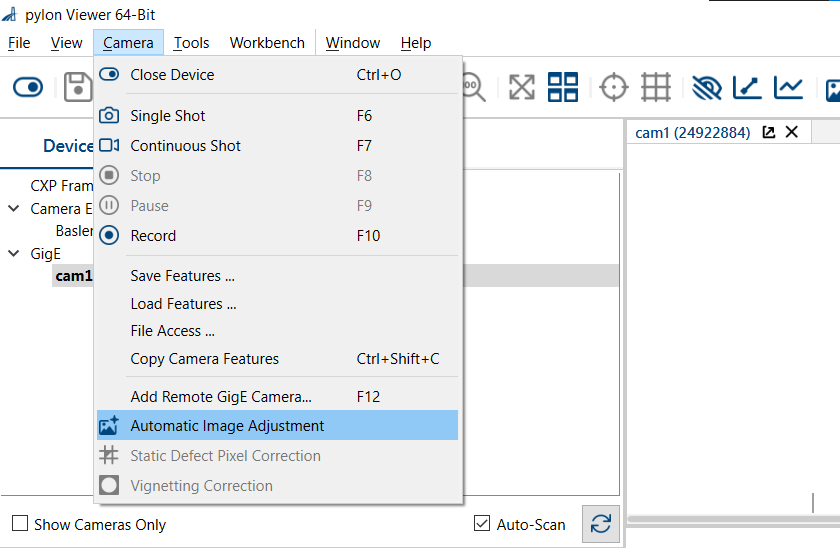
\includegraphics[width=1\linewidth]{figures/Chapter3/baslerauto.png}
        \caption{Cấu hình ảnh chụp}
        \label{c3:image}
 \end{figure}


% =======================
% PHẦN 3: XỬ LÝ ẢNH
% ======================= 
